\section{SLAM - Simultanious Localization And Mapping}
\label{chap:SLAM}
Als Simultaneous Localization and Mapping, auch \acs{SLAM}-Problem genannt, bezeichnet man die Aufgabe, die Trajektorie\footnote{Lösungskurve oder Bewegungspfad eines Objekts} 
samt Orientierungsinformation einer sich bewegenden Plattform, z.B. ein Smartphone, Tablet oder jegliche Art von Roboter, aus 
Beobachtungen zu schätzen und gleichzeitig aus den gewonnenen Informationen eine Karte der Umgebung zu erstellen.
Diese Aufgabe ist für den weiteren Prozess bedeutend. Zum einen sollen die generierten Karten sehr präzise sein, um einen hohen 
Wert für den Nutzer oder für spezielle auf der Karte aufbauende Anwendungen darzustellen. Zum anderen benötigen autonome Roboter, 
beispielsweise Saug- oder Mähroboter, ein solch erzeugtes geometrisches Modell der Umgebung, um zielgerichtet selbstständig navigieren zu 
können. %\cite{slamdefi.2016a} 
\begin{quote}
    Das Simultaneous Localization and Mapping oder kurz SLAM Problem behandelt das gleichzeitige Schätzen der Position und Ausrichtung einer 
    mobilen Plattform im Raum anhand der sich an Bord befindlichen Sensoren sowie den Aufbau eines Modells der Umgebung. Dieses Problem ist 
    von großer praktischer Relevanz und ist Kernbestandteil der meisten mobilen Sensorsysteme. \cite{slamdefi.2016a}
\end{quote}
1986 wurden auf der \textit{IEEE Robotics and Automation Conference} erste mathematische Definitionen vorgenommen, die mittels statischer 
Theorien ermittelt und mit ersten Studien belegt wurden. Einige Jahre später, im Jahr 1995, wurde das \acs{SLAM} Problem erstmals auf dem 
internationalen Symposium für Robotikforschung (\textit{ISRR'95}) vorgestellt. Die Forschungen hielten an, bis auf der \textit{ISRR'99} 
die erste \acs{SLAM} Sitzung stattfand. 

\subsection{Definition des Problems}
Angenommen ein Roboter startet in einer Position, auch Pose genannt, und einer Konfiguration \textit{p0} und bewegt sich durch eine ihm 
unbekannte Umgebung, stellen die nicht vorhandenen Kenntnisse seiner Position und der damit verbundenen Orientierung das Hauptproblem dar. 
Die Einstellung beinhaltet Position und Ausrichtung des Roboters. Je nach Bewegung in Raum oder Ebene ist die Pose meist als 3- oder 
6-dimensionaler Vektor abgebildet. Die Bewegung des 
Roboters wird durch bekannte Kontrollkommandos \textit{u} angewiesen, allerdings mit einer gewissen Unsicherheit versehen. Dabei wird 
zwischen den Zeitpunkten \textit{t-1} und \textit{t} die Bewegung des Roboters mit \textit{ut} beschrieben und somit auch die 
unterschiedlichen Posen \textit{pt-1} nach \textit{pt}. Die Umgebung wird parallel dazu über diverse Sensoren, z.B. interne Sensoren, bspw. 
Geschwindigkeits- oder Positionssensoren, und externer Sensoren, unter anderem Abstands- oder taktile Sensoren. Neben der Protokollierung der 
Position, bei der es zu Störungen oder Berechnungsfehlern kommen kann, gibt es Beobachtungen durch Sensoren die verrauscht, bzw. fehlerhaft 
sind und durch \textit{zt} angegeben werden.
\\ 
\linebreak
Mit diesen vorhandenen Werten ist die Schätzung der Trajektorie \textit{p0:T=[p0,p1,...,pT]T} des Roboters von Beginn der 
Fortbewegung bis zum Zeitpunkt \textit{T} das Ziel. Gleichzeitig zur Berechnung der Trajektorie wird eine Karte \textit{m} des Umfelds geschätzt, 
deren Darstellung den Anforderungen entsprechend angepasst werden kann. Mit den Anforderungen sind verschiedene Repräsentationen der Karten 
gemeint, darunter beispielsweise eine Veranschaulichung von Punktansammlungen an Gegenständen, gerenderte Oberflächenmodelle oder 
2D-Rasterkarten und verstärkt visualisierte 3D-Voxelkarten\footnote{(Zusammensetzung aus dem englischen volume \textit{vox} und elements 
\textit{el}), bez. einen Gitterpunkt in einem dreidimensionalen Gitter.}. Basierend auf den Sensormessintervallen \textit{z1:T} und den dabei
stattfindenden Kontrollkommandos \textit{u1:T} wird die Karte des Umfeldes und alle Positionen bestimmt. Die Wahrscheinlichkeitsverteilung 
\textit{p(p0:T,m|z1:T,u1:T)} wird durch die geschätzten Werte \textit{p0:T} und \textit{m} berechnet. 
\\ 
\linebreak
Die Berechnung der Wahrscheinlichkeitsverteilung ist auch unter dem Namen \textit{Offline-\acs{SLAM}} bekannt. In der Praxis ist allerdings 
die Schätzung der Position \textit{xt} und der Karte der Umgebung durch \textit{p(pt,m|z1:t,u1:t)} interessanter, da Roboter Entscheidungen 
basierend auf aktuellen Informationen, z.B. der Posenschätzung und dem Umgebungsmodell, treffen sollen. Die Variante der Echtzeitschätzung 
ist auch als \textit{Online-SLAM} bekannt. \cite{slamdefi.2016a}

\subsection{Localization}
Damit das Endgerät, Smartphone oder der Roboter seine Position in Erfahrung bringen und schätzen kann, werden Informationen und Möglichkeiten 
benötigt, die Bewegung in irgendeiner Form zu messen. Da das Nutzergerät eine eigene virtuelle Karte, unabhängig von der \acs{GPS}-basierten 
Position, generiert, ist das \textit{Tracking} über die Weltkoordinaten nicht Bestandteil des eigentlichen Verfahrens. Für die Erfassung der 
internen Systemzustände gibt es sogenannte interne Sensoren die in dem Roboter zur Verfügung stehen. Bestandteile dieser internen 
Sensorik sind unter anderem Positions-, Geschwindigkeits-, Beschleunigungssensoren und das \acl{INS}. Für die Positions- und 
Geschwindigkeitserkennung gibt es z.B. einen optischen Codierer, welcher durch Lichtimpulse die Geschwindigkeit als auch die zurückgelegte 
Strecke schätzen kann. Das \acs{INS} besteht aus Lagesensoren und einem Kreiselkompass (Gyroskop). Diese sind essentiell für die Bestimmung 
der Orientierung und Neigung des Geräts. Ausgehend von der Erdkugel beziehen sich diese Sensoren auf das gegebene inertiale Koordinatensystem.
Mittels \textit{Odometrie} können die von den Sensoren bereitgestellten Informationen über Position und Orientierung berechnet werden. Radgetriebene 
Systeme führen die Berechnung durch, da diese basierend auf dem Durchmesser des Rades ermittelt wird. In Kombination mit \textit{Koppelnavigation}\footnote{Engl. dead reckoning, ist die laufende Positionsbestimmung eines bewegten Objekts infolge der Bewegungsrichtung und Geschwindigkeit \cite{koppelnavigation.2019j}}
gilt dieses Verfahren für Roboter, bzw. Fahrzeuge auf Land, als Grundlage der Navigation. Durch die theoretische Berechnung werden 
Fehlerbetrachtungen, z.B. Verschleiß, Schlupf oder Unrundheit von Rädern, vernachlässigt und ist somit nicht als alleiniges Verfahren einzusetzen. \cite{robotik2.2020m}
\begin{align}
    \Delta U = \frac{\pi D}{\textit{n}C}N
\end{align}
Mit \textit{D} als Raddurchmesser, \textit{n} als Getriebeübersetzung, \textit{C} als Enkoderauflösung und \textit{N} als Anzahl der 
Enkoderimpulse wird die Positions- und Orientierung berechnet. 
\\ 
Smartphones berechnen die Fortbewegung über gegebene Sensoren, darunter Beschleunigungs- und Neigungssensoren und Gyroskop. Dieses Zusammenspiel an 
Sensoren ermöglicht die Wahrnehmung der Positionsveränderung und kann somit diese bestimmen.
\subsection{Mapping}
Um neben der Berechnung der Position durch die interne Sensorik die Umgebung registrieren und schätzen zu können, gibt es externe Sensoren, 
die sich mit der Erfassung der Umwelt beschäftigen. Auch hier gibt es viele Arten von Sensoren, mit denen es ermöglicht wird, die Umgebung 
wahrzunehmen. Darunter sind taktile Sensoren, Näherungs-, Abstands-, Positionssensoren und visuelle Sensoren. Hinsichtlich Abstandssensoren, die 
Messungen zwischen Gegenstand und Sensor durchführen, gibt es im Allgemeinen erhebliche Vorteile gegenüber den Näherungssensoren. Unter Anderem 
besitzen sie zum Beispiel eine größere Reichweite und ein größeres Blickfeld als Näherungssensoren. Somit können sie die Entfernung zu Gegenstände 
genauer ermitteln und geometrische Umweltinformationen besser erfassen. Für die Messung des Abstandes eignet sich die \ac{TOF}-Kamera, die 
mit dem Laufzeitverfahren Distanzen messen und berechnen kann. \cite{robotik2.2020m}
\\ 
Das Laufzeitverfahren funktioniert wie folgt:
\begin{align}
    \textit{d} = \frac{1}{2}\textit{ct}
\end{align}
Abstand zwischen der Zielfläche und dem Sensor \textit{d} ist das Produkt aus der Signalgeschwindigkeit \textit{c} und der messbaren Laufzeit 
\textit{t}. \cite{robotik2.2020m} Beispiele für solche \acs{TOF}-Kameras und deren Repräsentation sind folgender Abbildung (\ref{pic:tofCam}) zu entnehmen.
\begin{figure}[hbt!]
    \centering
    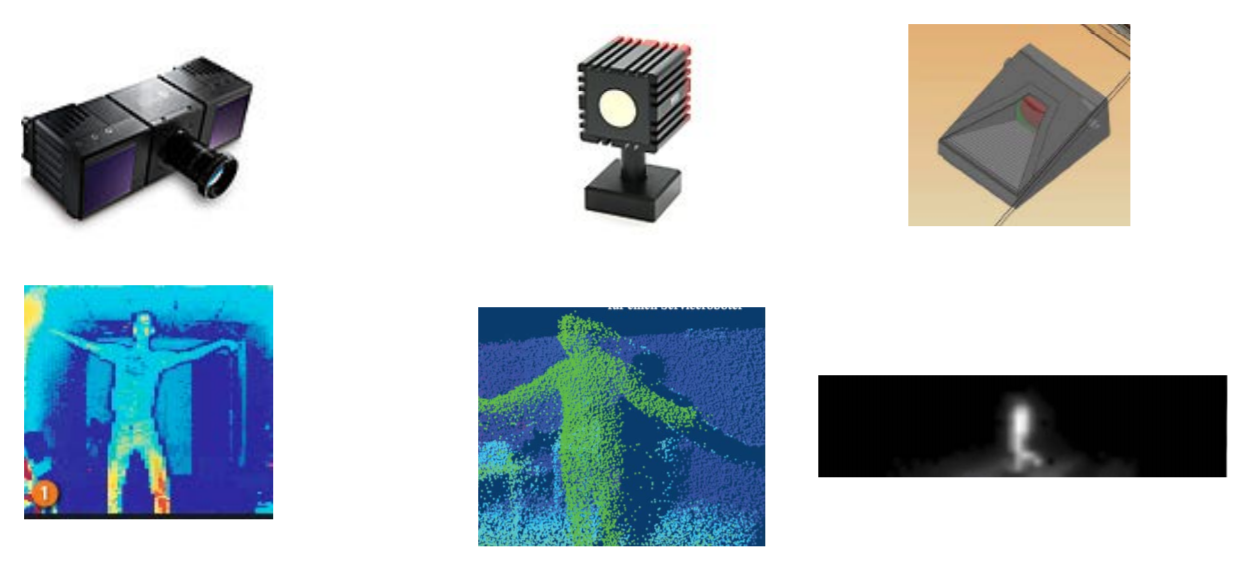
\includegraphics[width=13cm,height=13cm,keepaspectratio]{2Grundlagen/Bilder/tof_kamera.png}
    \caption{Time-of-Flight Kamera und deren Repräsentation \cite{robotik.2020m}}
    \label{pic:tofCam}
\end{figure}
\\ 
Auf der linken Seite ist eine PMD-Kamera\footnote{Photonic Mixing Device, optischer Sensor der auf dem Lichtlaufzeitverfahren beruht. Basiert auf dem TOF-Kameraprinzip} 
zu sehen, gefolgt von einer SwissRanger-Kamera und auf der rechten Seite eine IFM-Kamera\footnote{Eine erweiterte Art der 3D-Kamera}.

\subsection{Verfahren zur Lösung des SLAM Problems}
Das Lösen des \acs{SLAM} Problems wird in der Praxis mit den folgenden Verfahren, die sich bei der Anwendung bewährt haben, durchgeführt. In den 
folgenden Abschnitten werden zwei dieser Verfahren erläutert, sodass ein Grundverständnis der Funktionsweisen der Verfahren entsteht. 
Als Erstes erfolgt eine nähere Erläuterung des graph-basierten \acs{SLAM} Verfahren, gefolgt von der Lösung des Problems mit einem rekursiven 
Ansatz, dem erweiterten Kalman Filter (\acs{EKF}).

\subsection*{Graph-basiertes SLAM Verfahren}
Grundlegend wird bei dem Algorithmus des graph-basierten Verfahrens, während der Bewegungsaufzeichnung des Roboters, ein Graph modelliert, 
dessen Positionen zu verschiedenen Zeitpunkten durch Knoten dargestellt werden. Alle nebeneinander liegenden Positionen, bzw. Punkte, die 
lediglich minimale Unterschiede in der Umgebung aufweisen, werden zu einem Punkt gebündelt. Diese korrespondierenden Positionen, bzw. 
Knoten im Graphen werden über eine Kante verknüpft. Gebunden an die Bewegung des Roboters werden die Kanten modelliert. Der folgende Graph 
(\ref{pic:GraphSLAM}) veranschaulicht ein solches Modell.
\begin{figure}[hbt!]
    \centering
    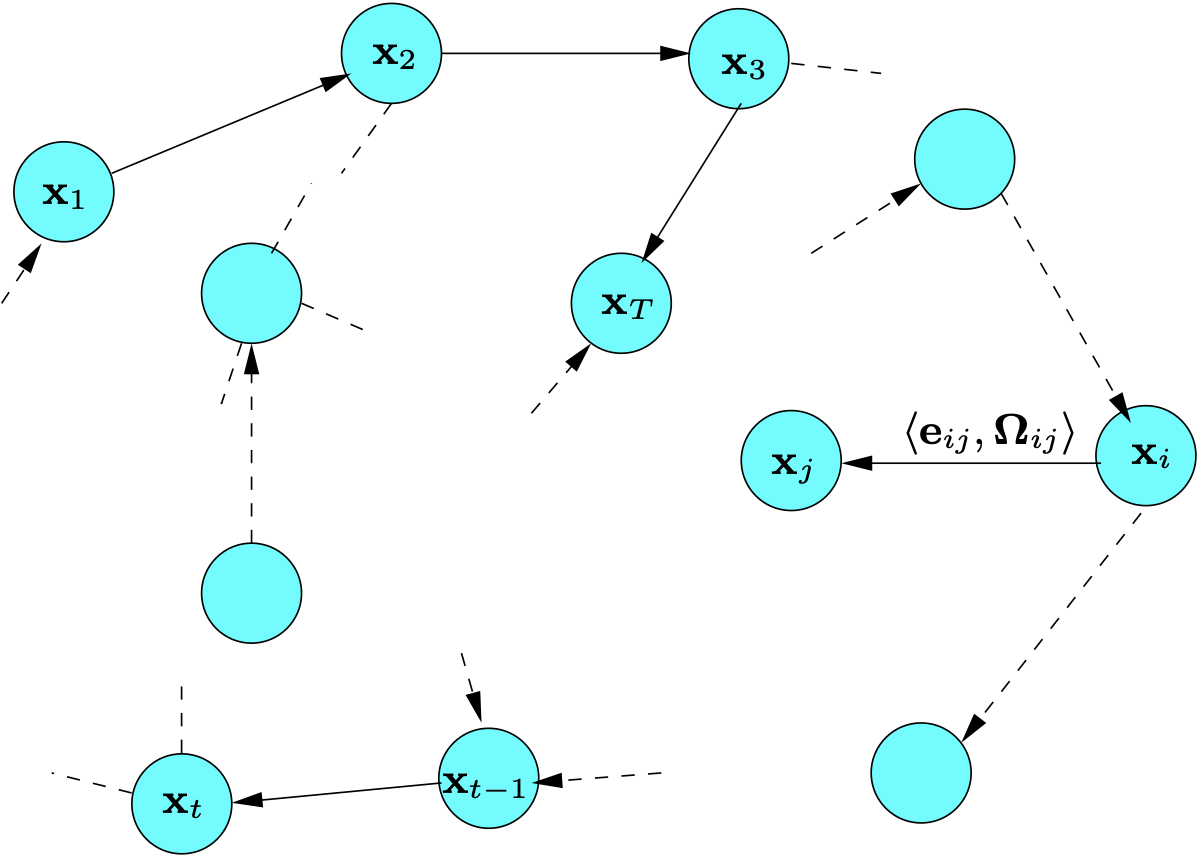
\includegraphics[width=10cm,height=10cm,keepaspectratio]{2Grundlagen/Bilder/graph_SLAM.png}
    \caption{Graphische Darstellung des SLAM Verfahrens \cite{graphSLAM.2010}}
    \label{pic:GraphSLAM}
\end{figure}
\\ 
Der Abbildung ist zu entnehmen, dass der Graph auch Kanten darstellt, die nicht den folgernden Knoten ansprechen, sondern eine 
Position vertreten, die in ihrer Beobachtung auf korrespondierende Knoten zurückgeht. Durch wiederholte Scans können genauere Merkmale und 
Bedingungen festgelegt werden, um die daraus resultierenden Positionen besser differenzieren zu können. Bei Verwendung von Kameras können 
genauer identifizierten Merkmale die geschätzten relativen Orientierungen sein, die durch eine zusätzliche Funktion berechnet werden 
können. Bei der Nutzung eines Lasersensors wird meist der \ac{ICP} Algorithmus angewendet, um die Veränderungen zwischen den Aufnahmepositionen 
wahrzunehmen. \acs{ICP} ist ein iteratives, ständig wiederholendes Verfahren, das die korrespondierenden Punkte schätzt und solange transformiert, bis diese unter 
einem gewissen Schwellwert liegen. Korrespondierende Punkte sind die, die den kleinsten Abstand zueinander haben (Closest Point). \cite{robotik2.2020m}
\\ 
Der inkrementelle Ansatz des graph-basierten \acs{SLAM} Verfahrens ist ursprünglich ein \textit{offline-Verfahren}, welches über die Jahre 
schrittweise zu einem \textit{online-Verfahren} führte. Durch diese ständige Beobachtung und Neuberechnung der aktuellen Position zu jedem 
Zeitpunkt wurde die Bedeutung der inkrementellen Verfahren gesteigert. %Dieser Ansatz ist besonders für monokulare Kameras ratsam und sinnvoll.

%\subsection*{Rekursives Schätzproblem}
%Der erweiterte Kalman-Filter (\acs{EKF}) ist eine wahrscheinlichkeitsbasierte rekursive Schätzung der Position des Objekts und der Position der 
%Landmarken unter Nutzung linearer Bewegungsmuster basierend auf dem Bayes-Filter. Der Bayes-Filter-Algorithmus ist das generelle Verfahren der 
%rekursiven Zustandsschätzung und wird über den Satz von Bayes\footnote{Mathematischer Satz der Wahrscheinlichkeitstheorie. Daruch wird die Berechnung einer bedingten Wahrscheinlichkeit beschrieben} 
%hergeleitet. 
%\\
%Unter der Voraussetzung einer Normalverteilung und eines linearen Bewegungsmodells, worauf der Kalman-Filter setzt, kann diese durch das 
%\acs{SLAM} Problem nicht erfüllt werden. An dieser Stelle wird der erweiterte Kalman-Filter eingesetzt, da dieser nicht-lineare 
%Bewegungsmodelle, bzw. Funktionen mittels Taylorreihe approximiert. Somit kann eine Messung in etwas vorhergesagt werden. Diese Schätzung 
%dient somit als Grundlage zur eigentlichen Messung. Nach der Berechnung wird der Zustand aktualisiert und ausgegeben. Mit diesem Ergebnis 
%werden die darauffolgenden Punkte rekursiv berechnet, bis die Scan-Phase zu Ende ist.
\section{Quaternionen}
\label{chap:Quaternionen} %\cite{quaternionHamilton.2006} 
Quaternionen, lat. \textit{„Menge der Vier“}, wurden erstmals 1843 von Sir William Rowan Hamilton beschrieben. Sie bezeichnen einen 
Zahlenbereich, der die reellen Zahlen erweitert. Die mathematische Formel wird häufig zur Darstellung einer Drehung im dreidimensionalen Raum 
verwendet. Die Theorie der Quaternionen basiert auf der mathematischen Grundlage der komplexen Zahlen, die 1833 von Hamilton als Bildung 
einer Algebra galten und werden daher als hyperkomplexe Zahlen aufgefasst.
\\ 
\linebreak
Mit \textit{a,b,c,d $\in q$} werden Quaternionen wie folgt beschrieben: \cite{quaternionRichter.2020m}
\begin{align}
    \textit{q} = \textit{a} + \textit{b} \cdot \textit{i} + \textit{c} \cdot \textit{j} + \textit{d} \cdot \textit{k}
\end{align}
In oben genannter Formel ist die Variable \textit{a} der Realteil und (\textit{b,c,d})$^T$ der Imaginärteil \textit{u} der Gleichung. 
Auch geschrieben als \textit{q = (a, u)$^T$}, um die Teile differenzieren zu können. 
\\ 
Mit der sogenannten \textit{Brougham Bridge}-Formel ist es möglich Vektoren zu dividieren. 
\begin{subequations}
    \label{Quaternionen-Gleichung}
    \begin{align}
        \textit{i$^2$} = \textit{j$^2$} = \textit{k$^2$} = \textit{ijk} = \textit{-1} 
        \label{erstes Gleichungsgesetz} \\
        \textit{ij} = \textit{-ji} = \textit{k} 
        \label{zweites Gleichungsgesetz} \\
        \textit{jk} = \textit{-kj} = \textit{i} 
        \label{drittes Gleichungsgesetz} \\ 
        \textit{i$^2$} = \textit{j$^2$} = \textit{j}
    \end{align}
\end{subequations}
\subsection{Rotation}
%\subsection{Transformation}
Quaternionen dienen als Möglichkeit, Drehungen, bzw. Rotationen darzustellen, unter anderem wegen der reduzierten Anzahl an 
benötigten Parametern im Vergleich zur Berechnung von Rotationsmatrizen und deren Translation. Die Quaternionen bieten eine deutlich kompaktere 
Darstellung der Rechenwege. Somit können Rotationen intuitiver veranschaulicht werden, d.h. es sind direkte Angaben von Drehwinkel und 
-achse möglich. Die kompaktere Darbietung beinhaltet lediglich vier Werte im Vergleich zu den neun Werten der Berechnung der Rotationsmatrix
und die Rotation kann um eine bestimmte Achse ermittelt werden. Zudem ist eine sehr hohe numerische Stabilität gewährleistet. 
\\ 
Der Drehwinkel wird wie folgt berechnet: \cite{quaternionRichter.2020m}
\begin{align}
    %\textit{a} = $\cos z$ \to \textit{z} = \frac{t}{2} \to t = $\theta$  %\textit{z} = \textit{\frac{$\theta$}{2}} 
    %\\
    \textit{$\theta$} = \textit{2} \cdot \textit{$\arccos a$}
\end{align}
Der Realteil \textit{a} des Quaternions wird mittels Arkuskosinus berechnet, so erhält man die Drehung des Objekts. Die Drehachse lässt sich 
bestimmen, indem alle Werte des Imaginärteils (\textit{b,c,d})$^T$ mit \textit{u} addiert werden. Die Variable \textit{u} setzt sich wie 
folgt zusammen:  \cite{quaternionRichter.2020m}
\begin{align}
    \textit{u} = \textit{$\sin w$}, \to \textit{w} = \frac{t}{2}, \to \textit{t = $\theta$}
\end{align}
Mit diesen zwei Berechnungen werden Drehwinkel und Drehachse bestimmt und können für weitere Berechnungen verwendet werden.
\\ 
\linebreak 
Die Orientierung eines feststehenden Körpers im dreidimensionalen euklidischen Raum kann auch mithilfe des Eulerschen Winkels beschrieben werden. Bei dieser 
Berechnung werden die Rotationsachsen und deren Reihenfolge festgelegt. Dabei wird der Abfolge entsprechend die Drehung um jeweils die veränderte Achse durchgeführt. 
Die Orientierungsbeschreibung wird mit 3x3-Matrix- oder homogenen 4x4 Matrix-Multiplikationen durchgeführt. Dabei ist das jeweilige Matrixprodukt die 
Grundlage für die weiteren Berechnungen der entstehenden Orientierung. \cite{quaternionRichter.2020m}
\begin{align}
    \textit{Rs} = \textit{Rz($\alpha$)} \cdot \textit{Ry'($\beta$)} \cdot \textit{Rz''($\gamma$)}
\end{align}
Die Formel beinhaltet die Matrix \textit{R} in jeweils gewandelter Form durch das linksstehende Matrixprodukt mit der Drehung durch den Winkel \textit{$\alpha$, $\beta$, $\gamma$}.
\\ 
\linebreak
Quaternionen sind im Vergleich zum Eulerschen Winkel übersichtlicher und kompakter in der Darstellung und Berechnung der Rotationen. \cite{quaternionRichter.2020m} 
Der Eulersche Winkel weist eine Unstetigkeit auf und ist für die allgemeine Rotationsbestimmung nicht eindeutig. \cite{euler.2000} Weiterer Nachteile des 
Eulerschen Winkels sind zum einen die getrennte Durchführung der Vektor- und Matrizenoperationen und zum Anderen die vielen Parameter, die zur Berechnung notwendig sind. 
Zudem kommt eine hohe Redundanz und die Interpolation ist durch die Winkelberechnung schwierig. \cite{quaternionRichter.2020m} 
